\section{最小绝对值回归性能优化}

\begin{frame}{交替凸优化算法的计算性能问题}
    \begin{itemize}
        \item
        交替凸优化算法需要求解多个最小绝对值回归问题,
        在变量较多情况下,线性规划算法计算性能较差。
    \end{itemize}
\begin{figure}[H]
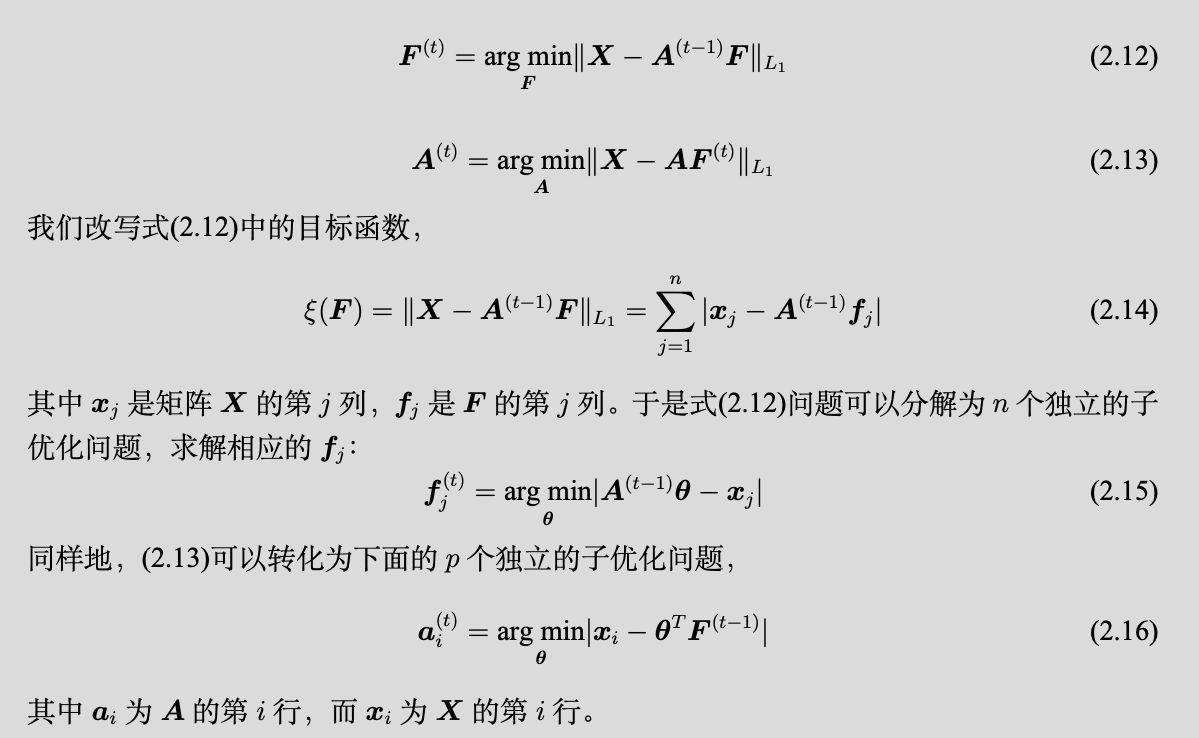
\includegraphics[width=8cm]{pics/acp-problem.png}
\end{figure}
\end{frame}

\begin{frame}{最小绝对值回归的优化1: 聚类——迭代拆解算法}
    \begin{itemize}
        \item
        Park等人于2016年提出一种聚类——迭代拆解算法,通过减小问题规模来提升计算性能。
    \end{itemize}
\begin{figure}[H]
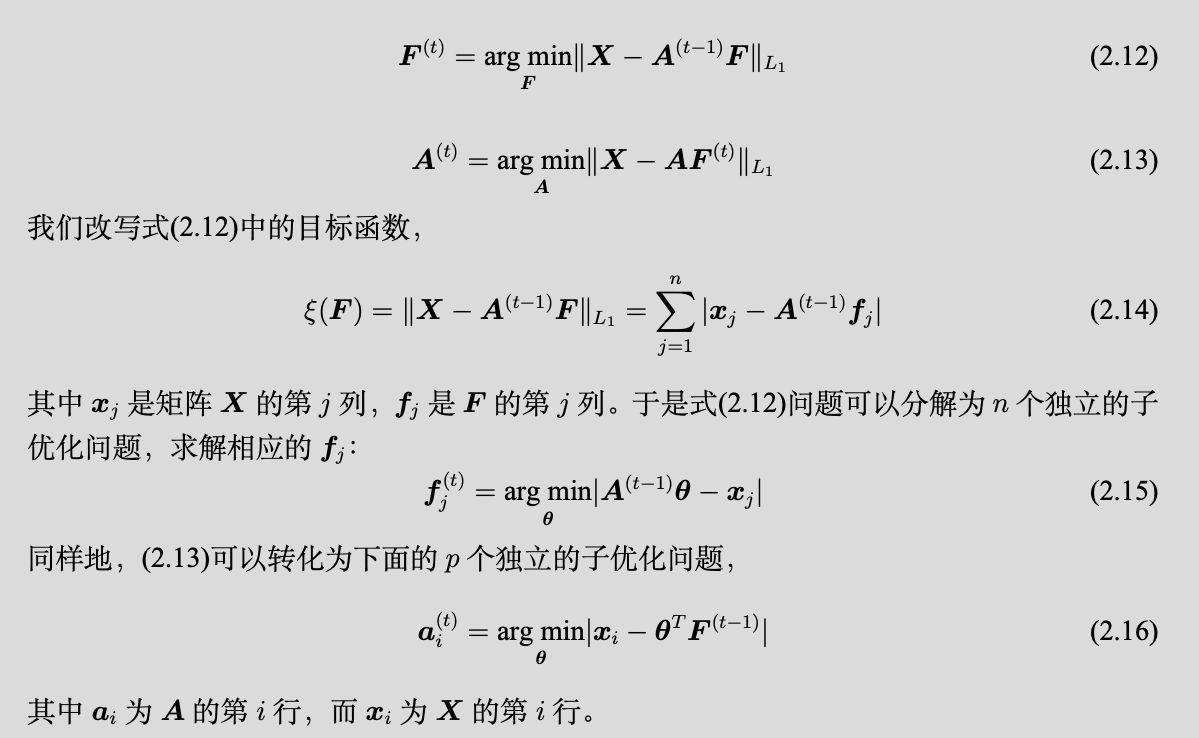
\includegraphics[width=8cm]{pics/acp-problem.png}
\end{figure}

\end{frame}
\begin{frame}{最小绝对值回归的优化1: 聚类——迭代拆解算法}
    \begin{itemize}
        \item 初始聚类,使用任意聚类方法,我们这里使用K-means。
    \end{itemize}
\begin{figure}[H]
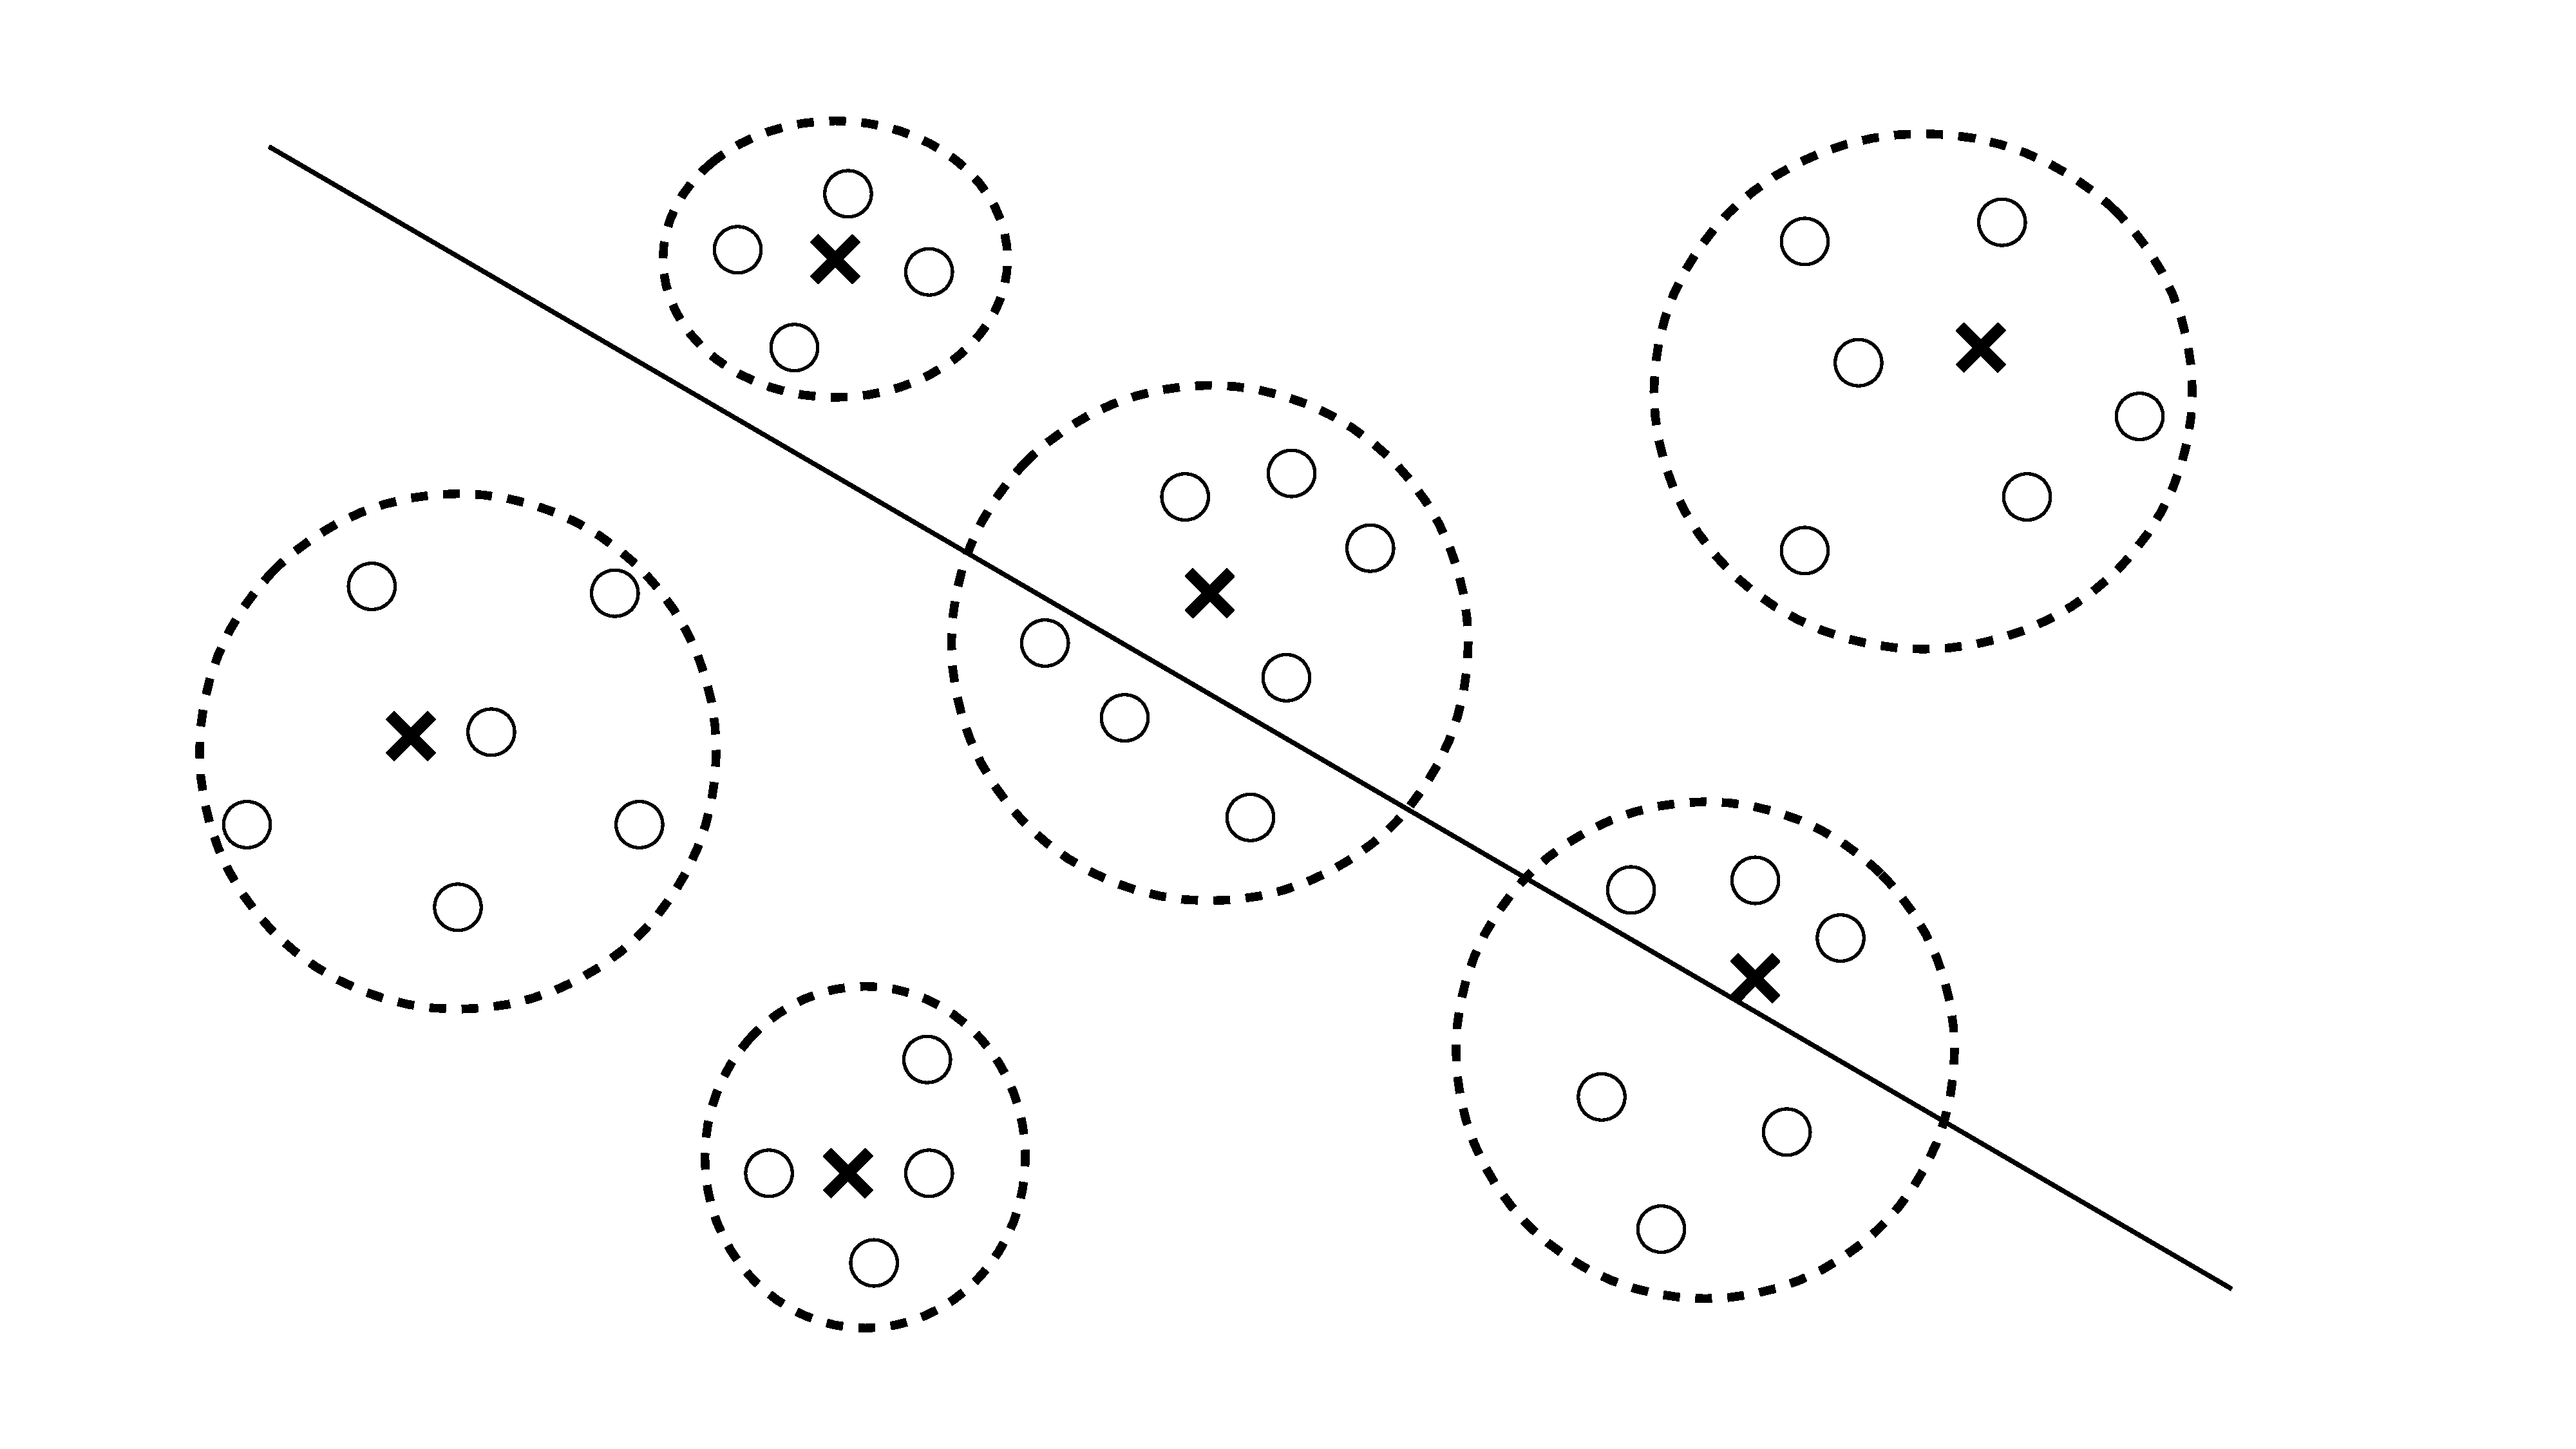
\includegraphics[width=10cm]{pics/aid-demo-a.pdf}
\end{figure}
\end{frame}

\begin{frame}{最小绝对值回归的优化1: 聚类——迭代拆解算法}
    \begin{itemize}
        \item 计算$\bm \beta$,按规则对聚类进行拆解。
    \end{itemize}
\begin{figure}[H]
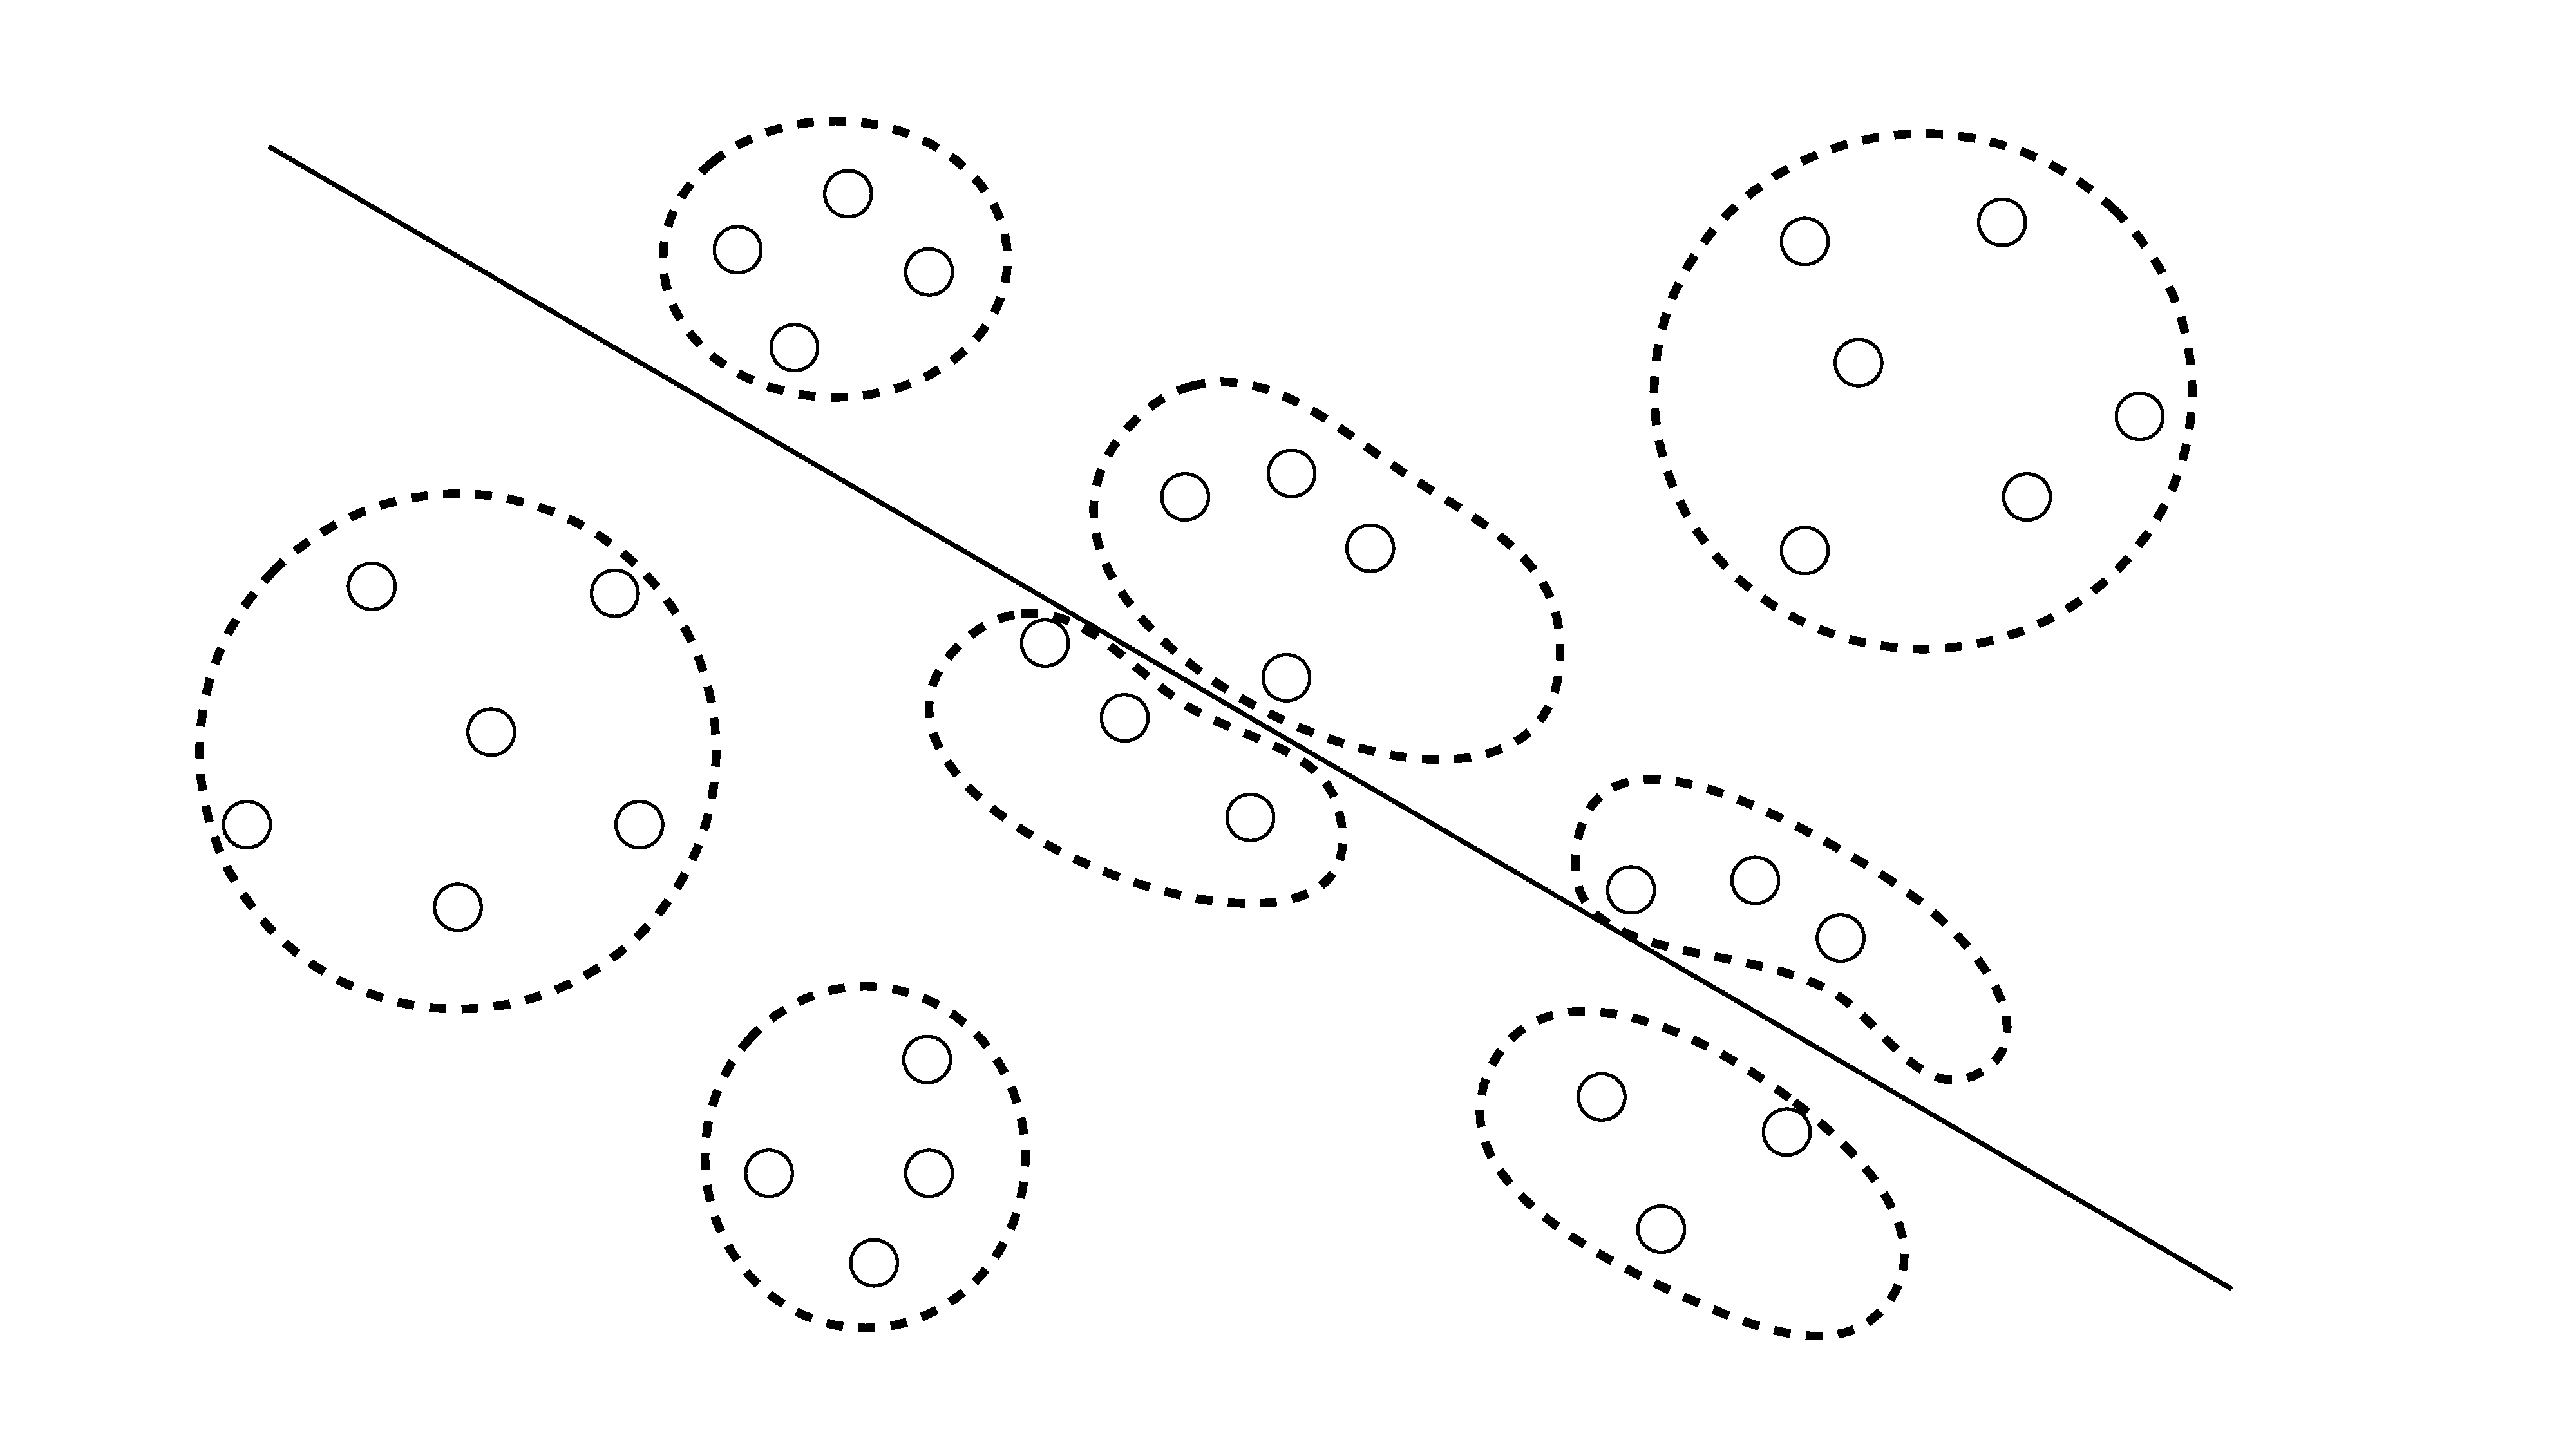
\includegraphics[width=10cm]{pics/aid-demo-b.pdf}
\end{figure}
\end{frame}

\begin{frame}{最小绝对值回归的优化1: 聚类——迭代拆解算法}
    \begin{itemize}
        \item 在新的聚类上重新计算$\bm \beta$。
    \end{itemize}
\begin{figure}[H]
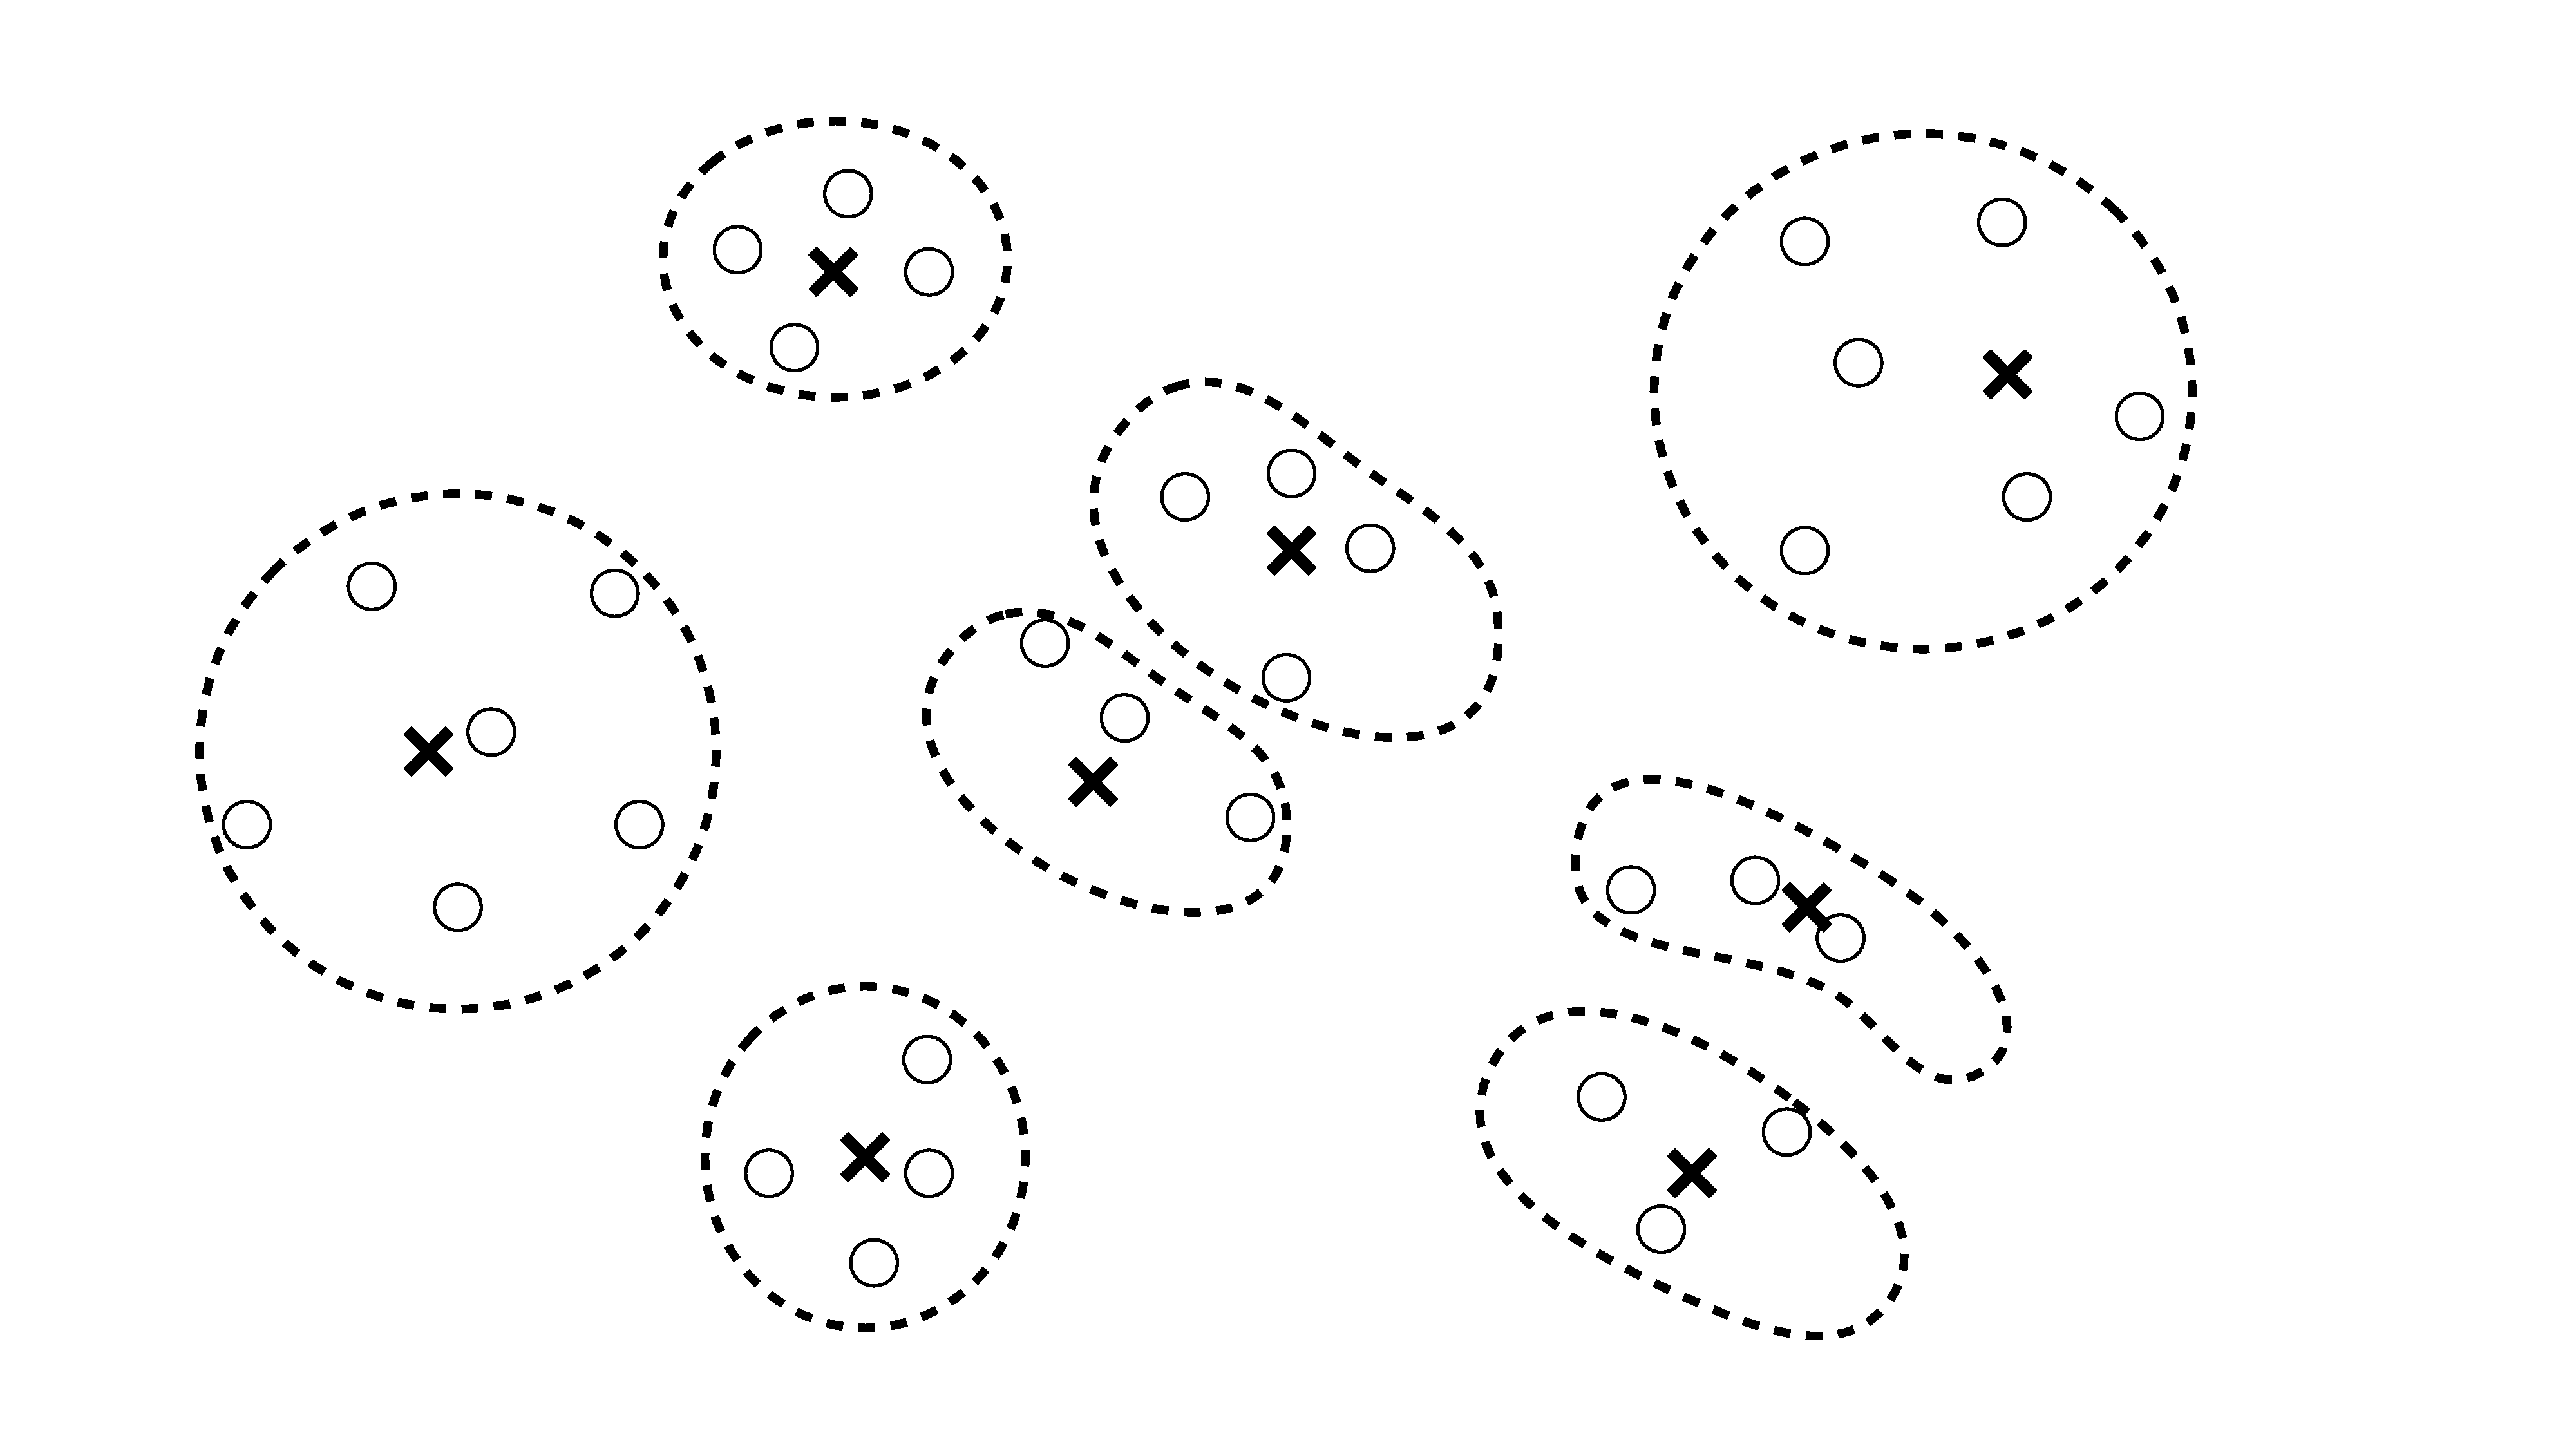
\includegraphics[width=10cm]{pics/aid-demo-c.pdf}
\end{figure}
\end{frame}

\begin{frame}{最小绝对值回归的优化1: 聚类——迭代拆解算法}
    \begin{itemize}
        \item 可以证明,该方法最终获得原问题的最优解
        (和在全部数据上解原优化问题有相同的解)。
    \end{itemize}
\begin{figure}[H]
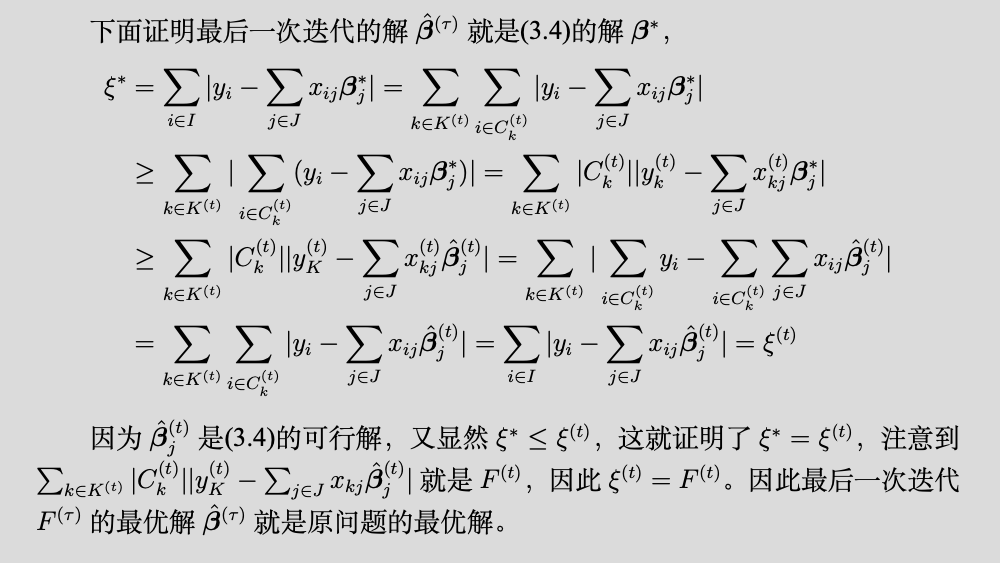
\includegraphics[width=10cm]{pics/proof-aid.png}
\end{figure}
\end{frame}